\section{Preparation phase}
\subsection*{Step 1}
The source eNodeB decides to initiate an Inter-RAT handover to the target access network.



\subsection*{Step 2}
The source eNodeB sends a \emph{Handover Required} message to the
source MME, requesting the CN to establish resources in the target RNC and in the
target SGSN. The message is sent through the S1 interface and it contains the
following parameters:
\begin{itemize}
	\item S1AP Cause: it specifies the reason of the message
	\item Target RNC Identifier: it identifies the target RNC
	\item CSG access mode: included only if the target cell is a hybrid cell
	\item CSG ID: included only if the target cell is a CSG or hybrid cell, it identifies the cell
	\item Source to Target Transparent Container: it carries RRC parameters and
	Radio Bearer information necessary to set-up the radio bearers.
\end{itemize}


\subsection*{Step 3}
The source MME determines from the ``Target RNC Identifier'' field that
the type of handover is intra-RAT Handover to UTRAN Iu mode and, if the CSG ID
is included in the message, it checks the UE's CSG subscribtion. If the UE isn't
subscribed to the CSG, then the MME rejects the handover, unless the UE has
emergency bearer services ongoing (in this case the handover to the target RNC is
performed independent of the restrictions).	If the handover isn't rejected then
the MME selects the target SGSN and sends to it	a \emph{Forward Relocation Request}
message through the S3 interface. Some of the parameters included in this message are:
\begin{itemize}
	\item user IMSI
	\item ISR Supported: it indicates if the source MME and the source S-GW are
	able to activate ISR\footnote{ISR = ``idle mode signalling reduction''. When
	this mode is active the network can simultaneously register the UE in a
	routing area that is served by an SGSN and in one or more tracking areas
	that are served by an MME.}
	\item PDN connections: it indicates the active PDN connections
	\item RAN cause: it's the S1AP cause received from the eNodeB
	\item CSG ID: included only if the target cell is a CSG cell or a hybrid cell
	\item CSG Membership Indication: it indicates if the UE is a CSG member. It's
	included only if the target cell is a hybrid cell or if it is a CSG cell and
	there is at least one emergency bearer service
	\item MM context: it includes information on the EPS Bearer\footnote{EPS Bearers
	= Bearers between the UE and the P-GW} contexts
	\item Source to Target Transparent Container
\end{itemize}
 If none of the UE's EPS Bearers is supported by the target SGSN, the source MME
 rejects the handover attempt and sends a Handover Preparation Failure message to the
 Source eNodeB (see chapter Handover Reject).


\subsection*{Step 4}
The target SGSN establishes the EPS Bearer contexts indicated by the message
received from the MME and deactivates the Bearer contexts which can't be
estabilished.

After that, it requests the target RNC to establish the radio
network resources (RABs) by sending the
\emph{Relocation Request} message through the Iu-PS interface. Some of the
parameters included in this message are:
\begin{itemize}
	\item Encryption information: it is sent in order to allow data transfer to
	continue in the new UTRAN target cell without requiring a new Authentication
	and Key Agreement (AKA) procedure
	\item RAB to be setup list: for each RAB to be set up it contains information
	such as the RAB ID (which contains the NSAPI value) and other RAB parameters
	\item CSG ID and CSG Membership Indication: included only when provided by
	the the source MME in the \emph{Forward Relocation Request} message
	\item Source RNC to Target RNC Transparent Container: it includes the information
	received from the source eNodeB included in the Source to Target Transparent
	Container field of the \emph{Handover required} message
\end{itemize}
If the target cell is a CSG cell, the target RNC verifies the CSG ID provided
by the target SGSN and rejects the handover if it does not match the CSG ID for
the target cell. If the CSG Membership Indication is ``non member'', the target
RNC only accepts emergency bearers.



\subsection*{Step 4a}
For each accepted bearer, the target RNC allocates radio and Iu
user plane resources. After that, the target RNC sends back to the SGSN the
\emph{Relocation Request Acknowledge} message, which contains a list of the
setup bearers and a list of the failed to setup bearers, which will be deactivated
by the SGSN.

After sending the ACK the RNC is prepared to receive downlink GTP
PDUs\footnote{Packets received by a protocol layer are called SDU while packets
output of a layer are called PDU.}
from the S-GW (or from the target SGSN if Direct Tunnel is not used) for the
accepted bearers.


%\subsection*{Step 6}
%\begin{figure}[!htb]
%	\centering
%	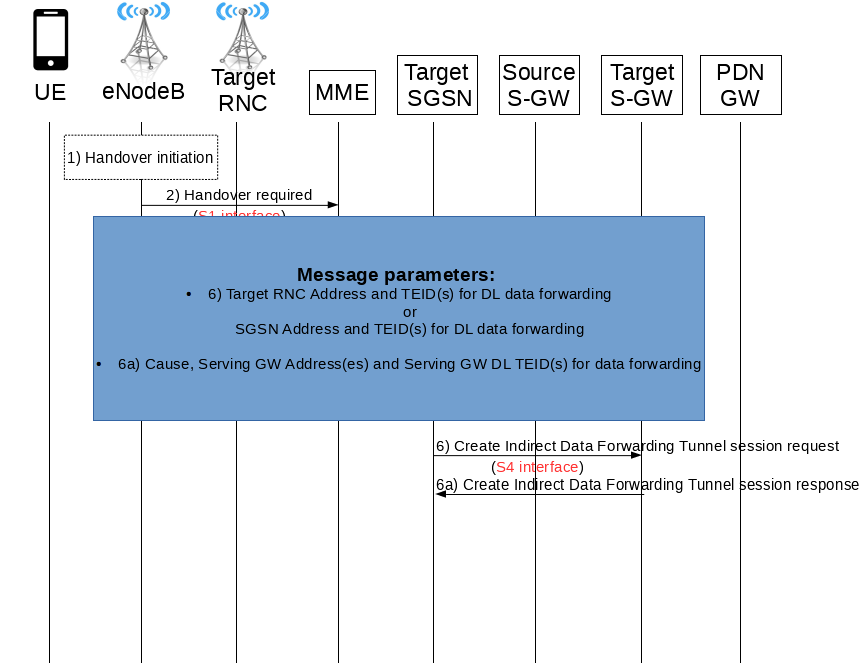
\includegraphics[width=0.9\linewidth]{img/6.png}
%	\label{fig:6}
%\end{figure}
%f Indirect Forwarding and relocation of S-GW apply then the
%target SGSN sends a \emph{Create Indirect Data Forwarding Tunnel Request}
%message to the target S-GW through the S4 interface. If GTP Direct Tunnel is used
%then message includes the Target RNC Address, while if Direct Tunnel isn't
%used the message includes the SGSN address. In both cases the message also
%include the TEIDs\footnote{TEID = Tunnel Endpoint identifier. Each GTP tunnel
%is associated with two TEID: one for the downlink and one for the uplink}
%for downlink user data forwarding.



%\subsection*{Step 6a}
%The S-GW responds to the SGSN with a \emph{Create Indirect Data Forwarding Tunnel
%Response} message, specifying as parameter the S-GW Address(es) and
%the S-GW DL TEID(s) for data forwarding.



\subsection*{Step 5}
The target SGSN sends the \emph{Forward Relocation Response} message
to the source MME through the S3 interface. Some of the parameters contained in
the message are:
\begin{itemize}
 \item Target to Source Transparent Container: it contains the value of the
 Target RNC to Source RNC Transparent Container received from the target RNC
 \item Address(es) and TEID(s) for User Traffic Data Forwarding: this field
 define the destination tunnelling endpoint for user data forwarding. If Direct Tunnel
 is used then it contains the addresses and GTP-U tunnel endpoint parameters
 to the Target RNC, otherwise it contains the DL GTP-U tunnel endpoint parameters
 to the Target SGSN.
 \item SGSN Tunnel Endpoint Identifier for Control Plane
 \item SGSN Address for Control Plane
\end{itemize}



\subsection*{Step 6}
If ``Indirect Forwarding'' applies, the Source MME sends the message \emph{Create
Indirect Data Forwarding Tunnel Request} to the S-GW used for indirect forwarding.
The parameters contained in the message are the list of ``Address(es) and TEID(s) for Data
Forwarding'' received in step 5 and the EPS Bearer ID(s).



\subsection*{Step 6a}
The S-GW replies sending message \emph{Create Indirect Data Forwarding Tunnel
Response}, which contains the S-GW Address(es) and the TEID(s) for data
forwarding. Note that the  Indirect Forwarding may be performed via a S-GW
which is different from the S-GW used as the anchor point for the UE.
If the S-GW doesn't support data forwarding, the message contains only an appropriate
cause.
